\Needspace{9in}
\begin{prob}

    Consider the following modification of BFS, with an added print statement:

    \begin{minted}[autogobble]{python}

        from collections import deque

        def modified_bfs(graph, source):
            """Start a BFS at `source`."""
            status = {node: 'undiscovered' for node in graph.nodes}
            status[source] = 'pending'
            pending = deque([source])

            while pending:
                u = pending.popleft()
                for v in graph.neighbors(u):
                    if v == 9:
                        print("Here!") # <-- this is the added print statement
                    if status[v] == 'undiscovered':
                        status[v] = 'pending'
                        pending.append(v)

                status[u] = 'visited'

    \end{minted}

    Consider running this algorithm on the following graph, starting at node $1$:

    \begin{center} 
    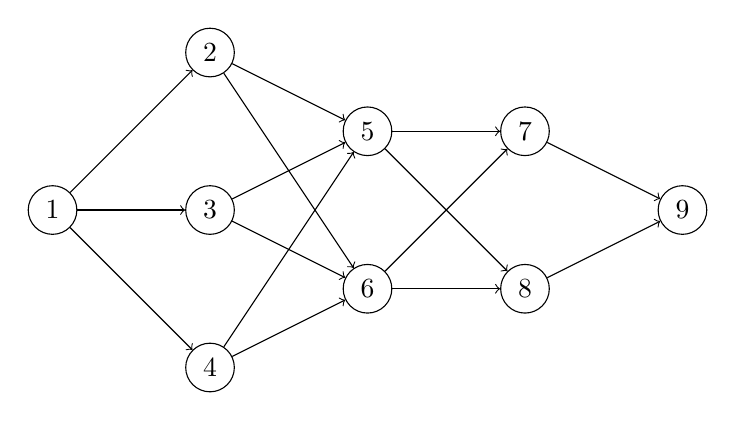
\begin{tikzpicture}

        \tikzset{every node/.style={circle, draw=black, minimum size=17pt}}

        \node (s) at (0, 0) {$1$};

        % nodes to the right, above right, and below right
        \node at (2, 2) (a) {2};
        \node at (2, 0) (b) {3};
        \node at (2, -2) (c) {4};

        % two nodes to the right, between the others
        \node at (4, 1) (d) {5};
        \node at (4, -1) (e) {6};

        % two nodes, directly to the right of d and e
        \node at (6, 1) (f) {7};
        \node at (6, -1) (g) {8};

        % last node
        \node at (8, 0) (x) {9};

        % edges, fully connected
        \draw[->] (s) -- (a);
        \draw[->] (s) -- (b);
        \draw[->] (s) -- (c);

        % second layer
        \draw[->] (a) -- (d);
        \draw[->] (a) -- (e);
        \draw[->] (b) -- (d);
        \draw[->] (b) -- (e);
        \draw[->] (c) -- (d);
        \draw[->] (c) -- (e);


        % third layer
        \draw[->] (d) -- (f);
        \draw[->] (d) -- (g);
        \draw[->] (e) -- (f);
        \draw[->] (e) -- (g);

        % last layer
        \draw[->] (f) -- (x);
        \draw[->] (g) -- (x);

    \end{tikzpicture}
    \end{center}

    How many times will \python{"Here!"} be printed?

    \inlineresponsebox[.75in]{2}


\end{prob}
